\section{Footstep Evaluation Network}

The purpose of the footstep evaluation network is to provide
candidate footstep positions to the GaitNet model. Importantly,
the exact costs output from this network are not critical, just that
they provide good candidate actions when sampled from. It accomplishes
this by ranking the cost of potential footstep positions given the
robot state. The architecture and training process are similar to
ContactNet \cite{bratta_contactnet_2024}, but with some key differences
detailed below.

%%%%%%%%%%%%%%%%%%%%%%%%%%%%%%%%%%%%%%%%%%%%%%%%%%%%%%%%%%%%%%%%%%%%%%%%%%%%%%%%
\subsection{Architecture}
\label{sec:contactnet-architecture}

The footstep evaluation network is tasked with generating a set of
footstep costs $\mathbf f_c$ based on $\mathbf x_c$:

\[
  \mathbf{x_c} =
  \begin{bmatrix}
    \mathbf p_{b,xy} \\
    \mathbf r_{w,z} \\
    \mathbf v_b \\
    \mathbf \omega_b \\
    \mathbf u
  \end{bmatrix}
\]

where
$\mathbf p_{b,xy}$ is the $x$ and $y$ position all end effectors in
the base frame stacked into a single vector, and
$\mathbf r_{w,z}$ is the height of the robot's COM in the world frame.
Here, the inclusion of $\mathbf \omega_b$ differs from
\cite{bratta_contactnet_2024}.

The model is trained on heuristically calculated footstep
cost maps (\autoref{fig:data-costmap-composition-combined}), which estimate
the cost associated with moving each foot to certain positions based on the
robot state.

The footstep evaluation network architecture is shown in
\autoref{fig:diagram-contactnet-architecture}. It consists of a
feedforward neural
network that first maps the input through two fully connected layers
of 64 nodes each, both with ReLU activations. The resulting 64-dimensional
feature vector is reshaped into an 8x8 spatial representation and
processed by a convolutional layer with two output channels, a
3x3 kernel, with stride 1, and padding 1, followed by a ReLU
nonlinearity. The output is flattened and passed to a final
fully connected layer before being reshaped into a 5x5 grid.

\begin{figure}[H]
  \centering
  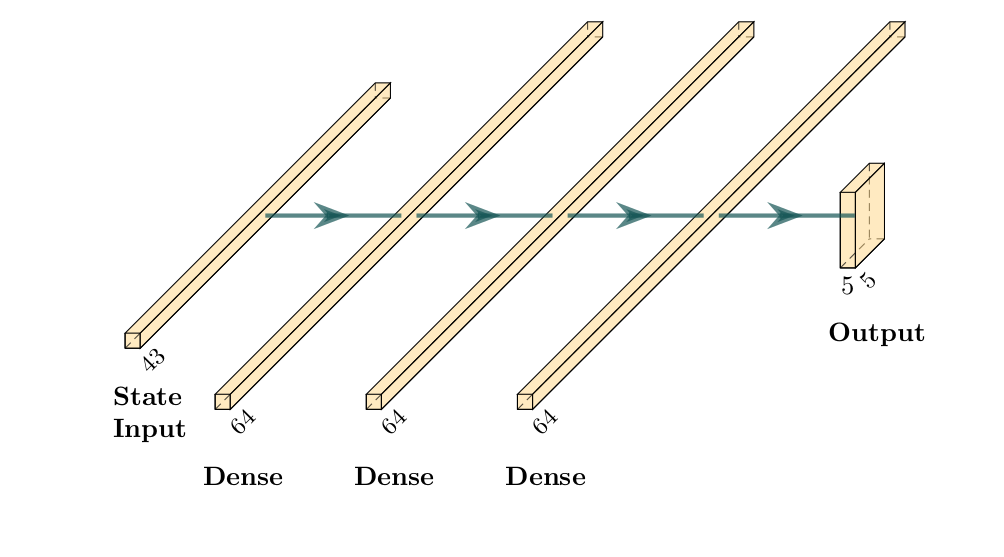
\includegraphics[width=0.5\linewidth]{images/diagrams/contact-network-architecture.png}
  \caption{Footstep evaluation neural network architecture.}
  \label{fig:diagram-contactnet-architecture}
\end{figure}

% \begin{figure}[H]
%   \centering
%   \includegraphics[width=0.5\linewidth]{images/data/footstep-cost-map.png}
%   \caption{Footstep cost map. Shows the heuristic cost for each
%   possible footstep location.}
%   \label{fig:data-footstep-cost-map}
% \end{figure}

%%%%%%%%%%%%%%%%%%%%%%%%%%%%%%%%%%%%%%%%%%%%%%%%%%%%%%%%%%%%%%%%%%%%%%%%%%%%%%%%
\subsection{Training}

The footstep evaluation network is trained to predict the heuristic
footstep cost maps used in \cite{bratta_contactnet_2024}. The training
data is generated in the simulation environment described in
\autoref{sec:simulation},
During the training sessions, 100 robots are run in parallel, being split
up into 4 groups of 25. Each group tests a grid of different footstep
positions for one foot at a time; the front left group is shown in
\autoref{fig:figure-training-fl-sweep}.
After every robot has finished (or failed) it's motion, an
\textit{iteration} is complete.
It is important to note that all robots start each iteration from the
same state.

\begin{figure}[H]
  \centering
  \includegraphics[width=0.5\textwidth]{images/figures/training-fl-sweep.png}
  \caption{Snapshot showing 25 robots testing different footstep
    positions in parallel. For real data generation, 100 are run in
  parallel, testing 25 footstep positions for each foot at a time.}
  \label{fig:figure-training-fl-sweep}
\end{figure}

During the data collection process, we chain together many
iterations, periodically
changing the control inputs. After each one,
the best 10 actions are placed into a tree structure as edges, with
the resultant
state as the leaf. The program then explores the tree by randomly selecting
leaves to expand. This process is repeated until a maximum number of
iterations is reached.
To avoid collecting poor data, iterations which result in more than
50\% of the robots falling
over are discarded, as well as their 2 parents up the tree. This
method ensures that a diverse
set of data is collected, while still focusing on the more successful
actions. \autoref{fig:data-cn-training-distribution}, shows
how the foot positions are distributed in the training data.
The darker spots are the discrete points which are used as candidate
footstep positions. For any given datapoint a foot is in one of these
positions because it was just moved there.

\begin{figure}[H]
  \centering
  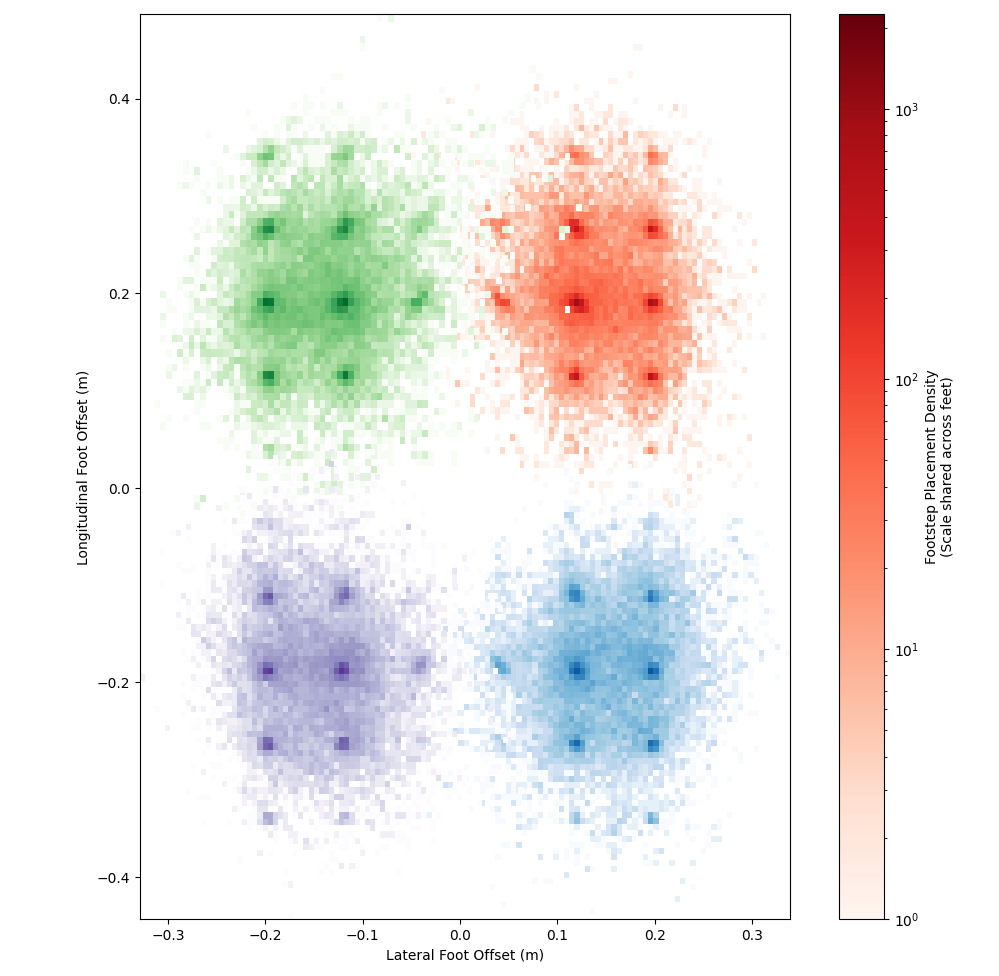
\includegraphics[width=0.5\textwidth]{images/data/foot-placement-heatmaps.png}
  \caption{Foot placement heatmaps showing distribution of foot
    positions in the GaitNet training data. Note that the histograms
  are overlaid in some places, obscuring data underneath.}
  \label{fig:data-cn-training-distribution}
\end{figure}

The purpose of this data collection is to generate the associated cost of
moving a foot to a specific position, a set of $\mathbf f_c$. The \textit{cost}
of each footstep position is calculated heuristically from the simulations.
The heuristic was designed to encourage a balance of stability and efficiency.
The specific factors that make up the footstep cost maps in the training data
are shown in \autoref{fig:data-costmap-composition-elements}, while the
combined cost map is shown in \autoref{fig:data-costmap-composition-combined}.
The factors are justified below.

\begin{itemize}
  \item \textit{lin\_vel\_z\_l2}\textemdash Penalizes high vertical
    velocity of the trunk.
  \item \textit{ang\_vel\_xy\_l2}\textemdash Penalizes high angular
    velocity of the trunk in
    the horizontal axes.
  \item \textit{joint\_torques\_l2}\textemdash Penalizes high joint torques.
  \item \textit{joint\_acc\_l2}\textemdash Penalizes high joint accelerations.
  \item \textit{control\_error}\textemdash Penalizes errors between the control
    input and actual robot motion.
  \item \textit{inscribed\_circle\_radius}\textemdash Measures the distance
    from the COM to the nearest edge of the support polygon. This
    encourages the robot to keep its COM in a stable position.
  \item \textit{foot\_hip\_distance}\textemdash Measures the distance from
    the nominal foot position. This encourages the robot to keep its feet
    moving along with the body.
\end{itemize}

\begin{figure}[H]
  \centering
  \begin{subfigure}[T]{0.65\textwidth}
    \centering
    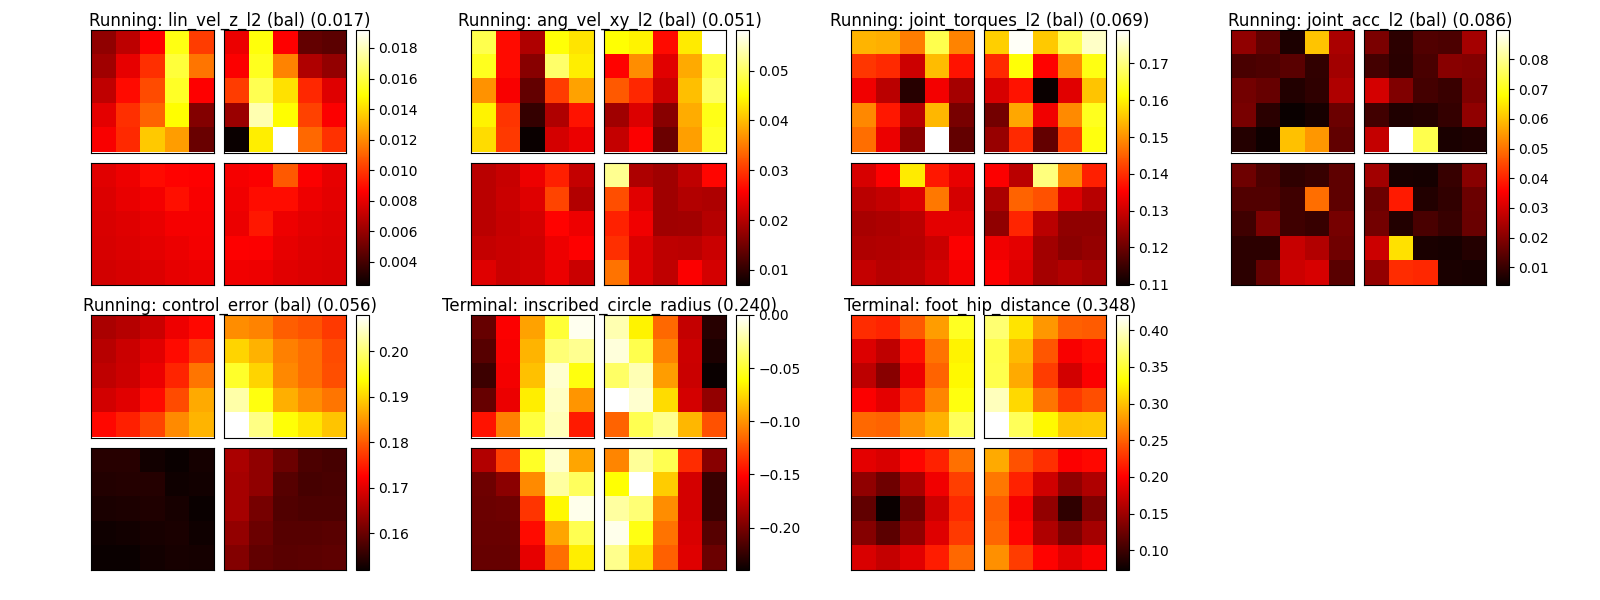
\includegraphics[width=\textwidth]{images/data/training/costmap-composition/elements.png}
    \caption{Factors influencing footstep cost maps. \textit{(bal)}
      indicates that the values for each leg were balanced to have a
      lower spread, mitigating factors that consistently prefer one leg
      over another. The last number in parenthesis indicates the total
    range of the data, the most important factor for the combined cost map.}
    \label{fig:data-costmap-composition-elements}
  \end{subfigure}
  \hfill
  \begin{subfigure}[T]{0.3\textwidth}
    \centering
    \includegraphics[width=\textwidth]{images/data/training/costmap-composition/combined.png}
    \caption{Combined cost map from factors in (a) (not normalized).}
    \label{fig:data-costmap-composition-combined}
  \end{subfigure}
  \hfill
  \caption{Footstep cost map composition. (a) shows the individual
    factors that make up the footstep cost maps, while (b) shows the
  combined cost map.}
  \label{fig:data-costmap-composition}
\end{figure}

As in \cite{bratta_contactnet_2024}, the cost maps are normalized to
improve training performance. Our approach differs in how the cost
maps are normalized though. We directly normalize the cost maps to
the range $[0, 1]$, whereas \cite{bratta_contactnet_2024} normalizes
to $[0,1]$ in such a way that only the relative ordering of costs are
preserved. This difference is critical to our system to provide the
upstream GaitNet model with as much information as possible.

%%%%%%%%%%%%%%%%%%%%%%%%%%%%%%%%%%%%%%%%%%%%%%%%%%%%%%%%%%%%%%%%%%%%%%%%%%%%%%%%
\subsection{Post-Processing}

Ultimately, the purpose of the footstep evaluation network is to
provide candidate footstep positions to the GaitNet model.
\autoref{fig:diagram-costmap-processing} shows the processing pipeline.
The raw cost map output (\autoref{fig:diagram-costmap-processing-raw})
from the footstep evaluation network is first upsampled
(\autoref{fig:diagram-costmap-processing-upsample}) to increase the
resolution of possible footstep positions, and to match the resolution of
the terrain data. Next, noise is added
(\autoref{fig:diagram-costmap-processing-noise}) to
encourage exploration of more varied footstep positions. Without noise,
all of the candidate footstep positions would be right next to each other.
The cost map is then filtered based on the robot state and terrain data
(\autoref{fig:diagram-costmap-processing-cspace}) to mask out
invalid actions, including positions that are too close to terrain edges,
and actions which would attempt to move a leg already in the swing state
(seen in the Front Right leg in this figure). Finally, the top 8
candidates from each leg are selected
(\autoref{fig:diagram-costmap-processing-topk})
to be processed by GaitNet. In the case where there are fewer than 8 valid
candidates for a leg, no-action candidates are added to the set to maintain
the size of the tensors.

% === Define layout constants ===
\def\imgwidth{0.16\textwidth}
\def\xgap{2em}          % horizontal gap between images
\def\arrowwidth{1.2em}  % controls arrow length
\def\arrowshift{0.5em} % vertical offset of arrows

\begin{figure}[H]
  \centering
  \begin{tikzpicture}[node distance=\xgap, baseline=(current bounding
    box.center)]

    % === Style for image blocks ===
    \tikzset{
      imgblock/.style={inner sep=0pt, outer sep=0pt, align=center}
    }

    % === Subfigure nodes ===
    \node[imgblock] (a)
    {\subcaptionbox{Raw\label{fig:diagram-costmap-processing-raw}}%
    {\includegraphics[width=\imgwidth]{images/diagrams/cost-map-processing/1-default.png}}};

    \node[imgblock, right=of a]
    (b)
    {\subcaptionbox{Upsample\label{fig:diagram-costmap-processing-upsample}}%
    {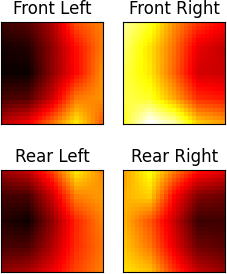
\includegraphics[width=\imgwidth]{images/diagrams/cost-map-processing/2-upscale.png}}};

    \node[imgblock, right=of b]
    (c)
    {\subcaptionbox{Noise\label{fig:diagram-costmap-processing-noise}}%
    {\includegraphics[width=\imgwidth]{images/diagrams/cost-map-processing/3-noise.png}}};

    \node[imgblock, right=of c]
    (d)
    {\subcaptionbox{C-space\label{fig:diagram-costmap-processing-cspace}}%
    {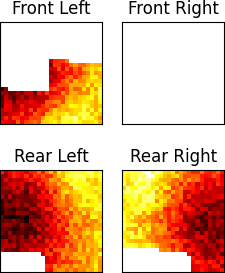
\includegraphics[width=\imgwidth]{images/diagrams/cost-map-processing/4-masked.png}}};

    \node[imgblock, right=of d]
    (e)
    {\subcaptionbox{TopK (green)\label{fig:diagram-costmap-processing-topk}}%
    {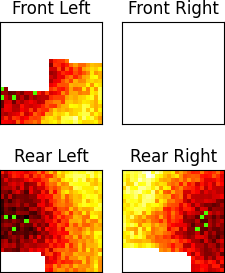
\includegraphics[width=\imgwidth]{images/diagrams/cost-map-processing/5-selected.png}}};

    % === Arrows ===
    \foreach \src/\dst in {a/b, b/c, c/d, d/e}{
      \draw[->, thick] ([yshift=\arrowshift]\src.east) --
      ++(\arrowwidth,0) --
      ([yshift=\arrowshift]\dst.west);
    }

  \end{tikzpicture}

  \caption{Cost map processing pipeline. Shows how the raw cost map
  is processed to produce the final footstep candidates.}
  \label{fig:diagram-costmap-processing}
\end{figure}
